\documentclass{beamer}

\usepackage[utf8]{inputenc}
\usepackage{hyperref}

\usetheme{Berkeley}
\beamertemplatenavigationsymbolsempty
\setbeamertemplate{headline}{}
 
\title{Creating a Workflow in FoodChain-Lab 1}
\date{}
 
\begin{document}
\maketitle

\section{ }
 
\subsection{1}
\begin{frame}
	\begin{center}
  		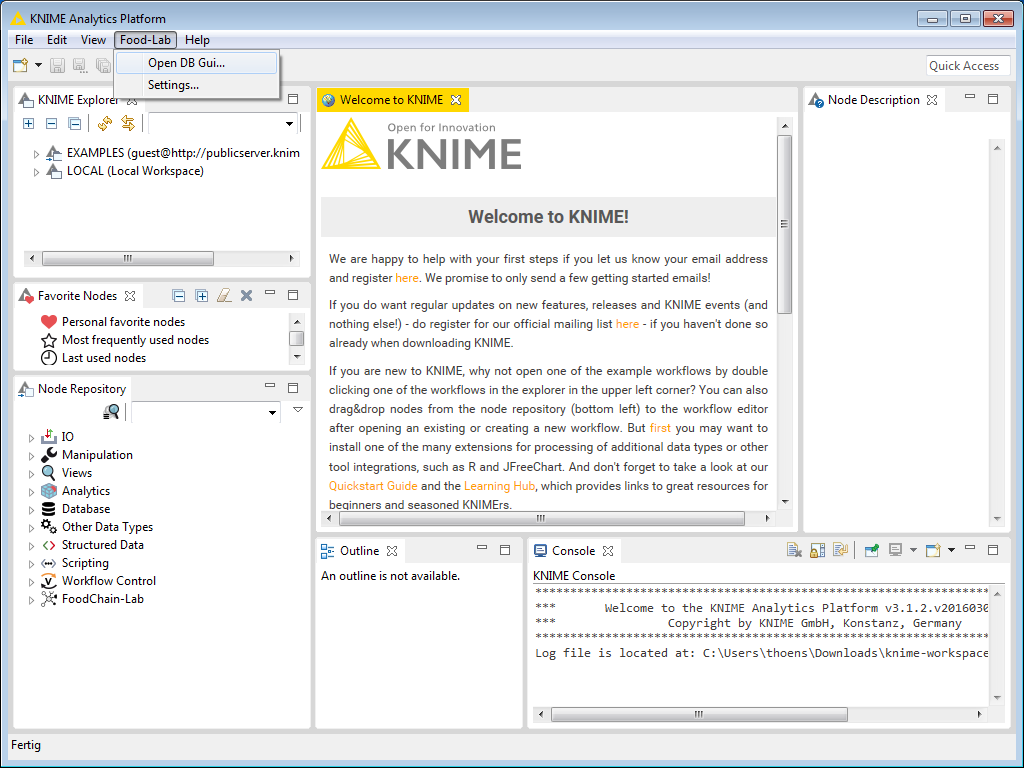
\includegraphics[height=0.6\textheight]{1.png}
	\end{center}
	\begin{itemize}
		\item Select \textbf{Food-Lab $>$ Open DB Gui...} in the menu bar to open the database dialog.
	\end{itemize}
\end{frame}

\subsection{2}
\begin{frame}
	\begin{center}
  		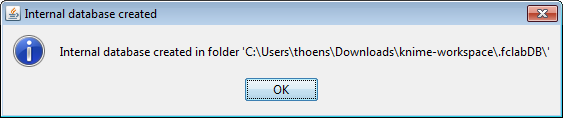
\includegraphics[width=0.9\textwidth]{2.png}
	\end{center}
	\begin{itemize}
		\item If you get a message saying the internal database has been created, click \textbf{OK}.
	\end{itemize}
\end{frame}

\subsection{3}
\begin{frame}
	\begin{center}
  		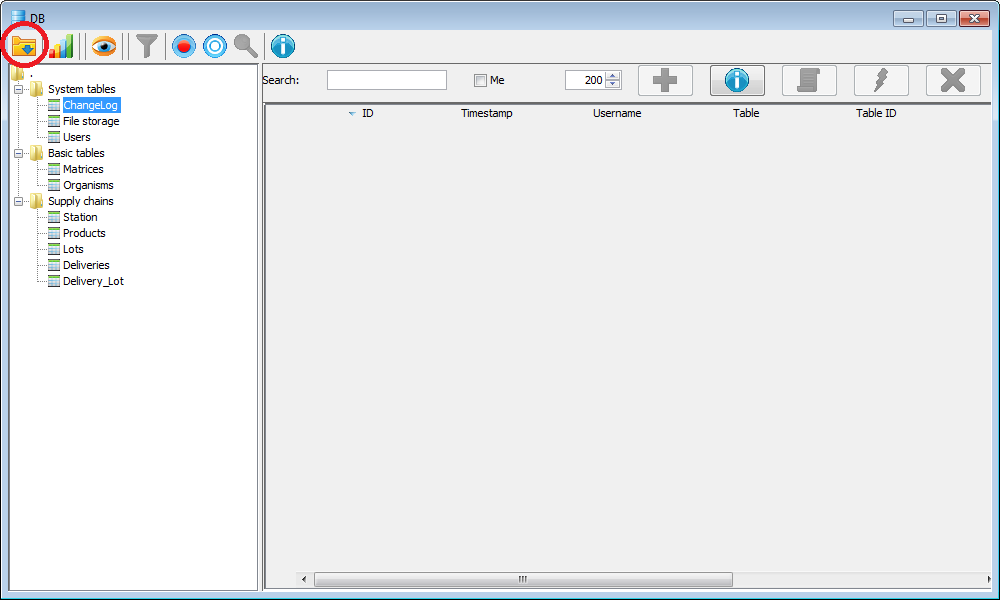
\includegraphics[height=0.6\textheight]{3.png}
	\end{center}
	\begin{itemize}
		\item In the database dialog click the \textbf{Table import} button in the upper left corner.
	\end{itemize}
\end{frame}

\subsection{4}
\begin{frame}
	\begin{center}
  		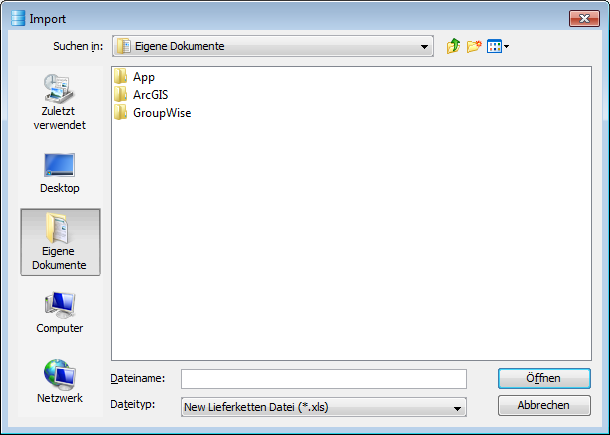
\includegraphics[height=0.6\textheight]{4.png}
	\end{center}
	\begin{itemize}
		\item Now a file dialog will pop up.
		\item *.xls files in FoodChain-Lab format can be selected here.
	\end{itemize}
\end{frame}

\subsection{5}
\begin{frame}
	\begin{center}
  		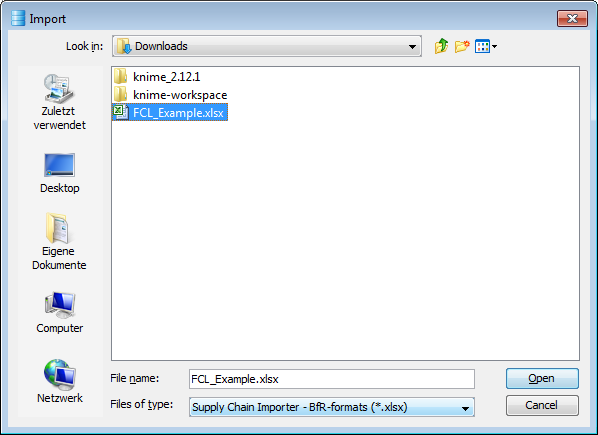
\includegraphics[height=0.6\textheight]{5.png}
	\end{center}
	\begin{itemize}
		\item Download the example file from \url{https://github.com/SiLeBAT/BfROpenLabResources/raw/master/GitHubPages/documents/fake_data.xls}.
		\item Select the file in the dialog and press \textbf{Open}.
	\end{itemize}
\end{frame}

\subsection{6}
\begin{frame}
	\begin{center}
  		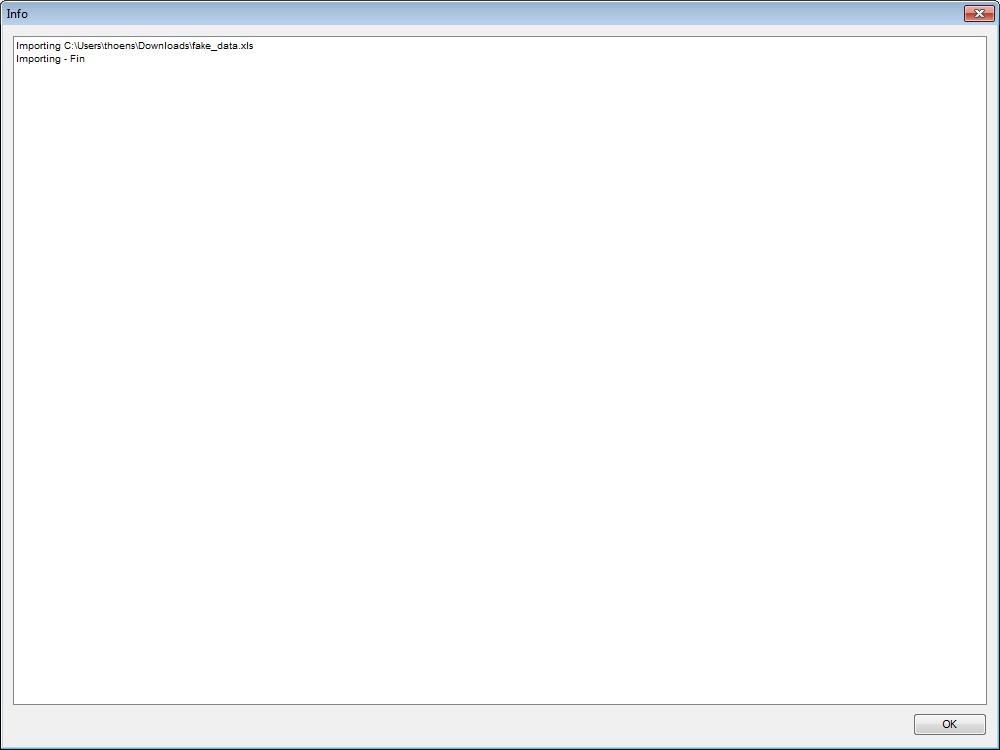
\includegraphics[height=0.6\textheight]{6.png}
	\end{center}
	\begin{itemize}
		\item When the importing is finished you see a dialog with errors/warnings,  that occurred in the import process.
		\item No errors ocurred, so just press \textbf{OK}.
	\end{itemize}
\end{frame}

\subsection{7}
\begin{frame}
	\begin{center}
  		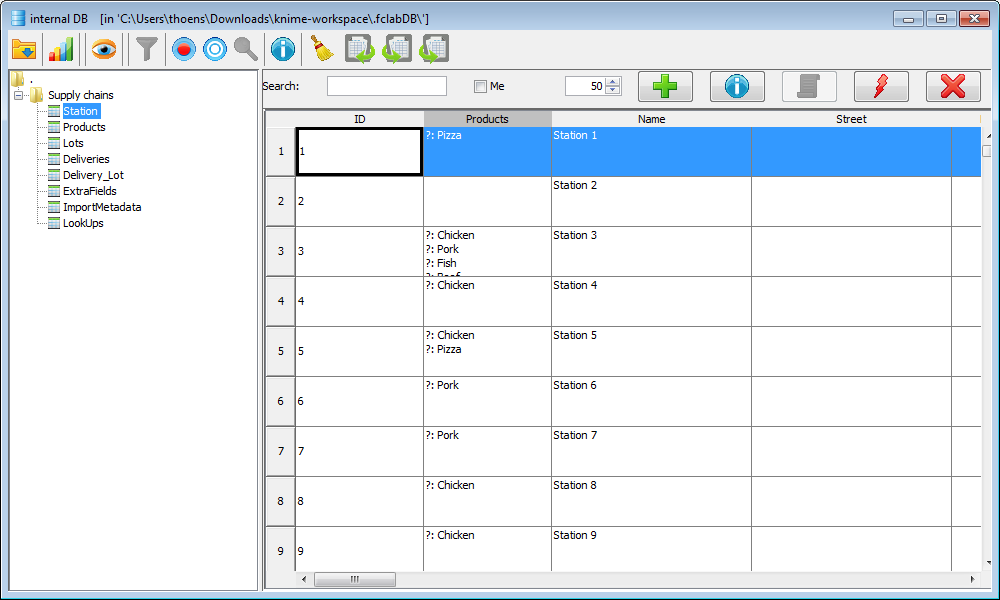
\includegraphics[height=0.6\textheight]{7.png}
	\end{center}
	\begin{itemize}
		\item In the database dialog, you can now look at the imported data and check the data for duplicates.
		\item Close the dialog.
	\end{itemize}
\end{frame}

\subsection{8}
\begin{frame}
	\begin{center}
  		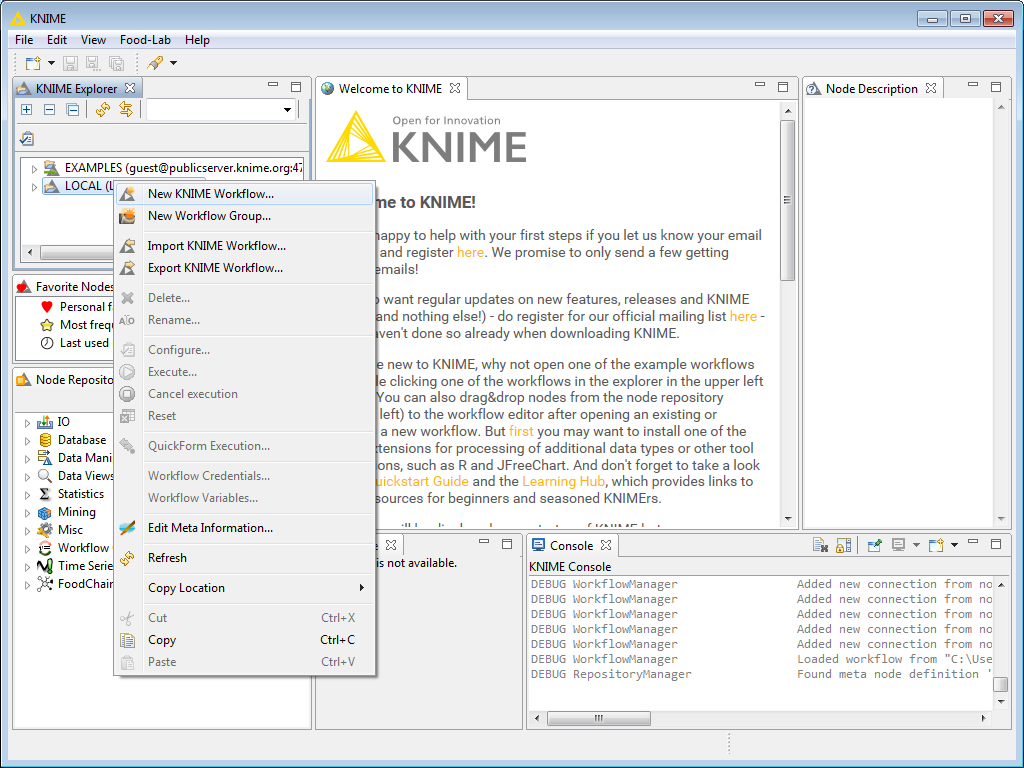
\includegraphics[height=0.6\textheight]{8.png}
	\end{center}
	\begin{itemize}
		\item Now we want to create a workflow, that uses the imported data.
		\item Right click on \textbf{LOCAL} in the \textbf{KNIME Explorer} and select \textbf{New KNIME Workflow...}
	\end{itemize}
\end{frame}

\subsection{9}
\begin{frame}
	\begin{center}
  		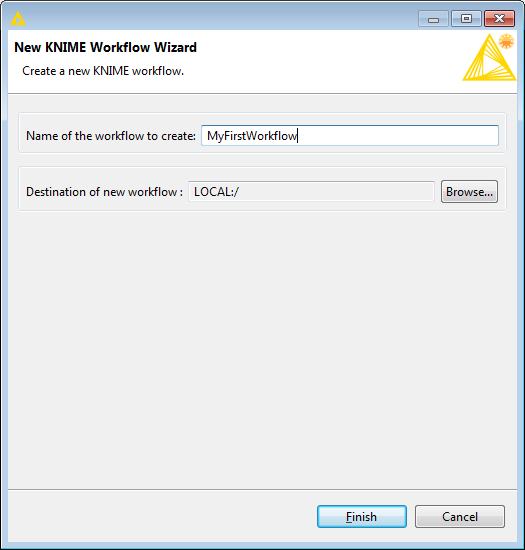
\includegraphics[height=0.6\textheight]{9.png}
	\end{center}
	\begin{itemize}
		\item In the dialog set the name of the workflow to "My First Workflow" and click \textbf{Finish}.		
	\end{itemize}
\end{frame}

\subsection{10}
\begin{frame}
	\begin{center}
  		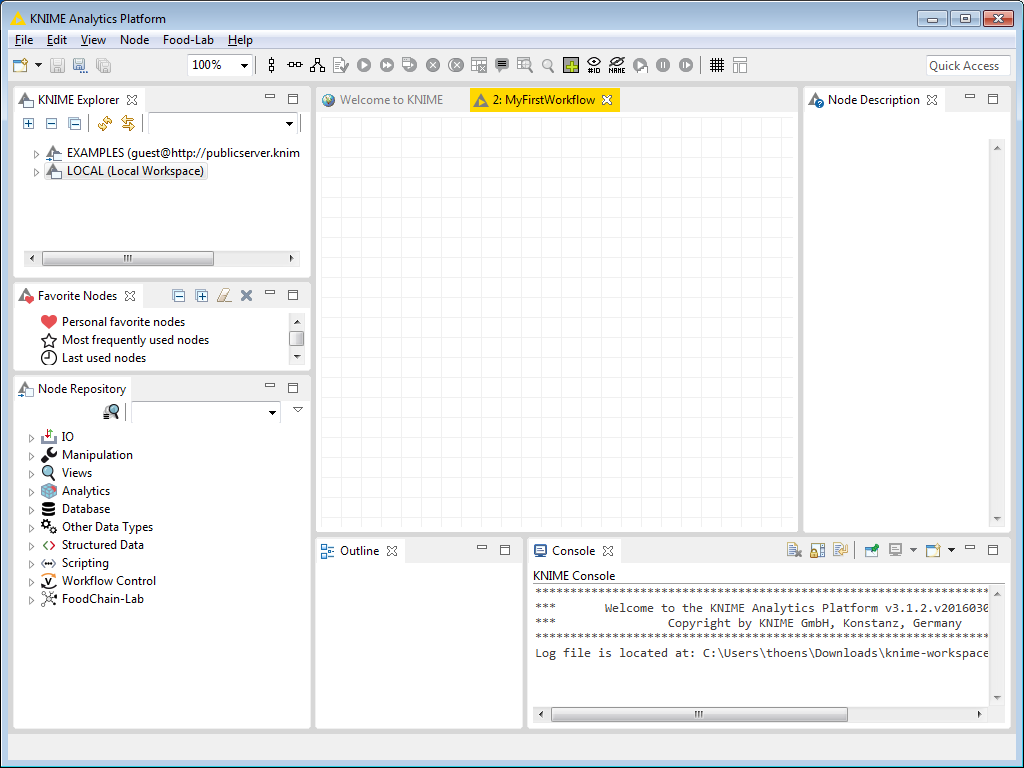
\includegraphics[height=0.6\textheight]{10.png}
	\end{center}
	\begin{itemize}
		\item The created workflow will shop up in the editor in the center.
	\end{itemize}
\end{frame}

\subsection{11}
\begin{frame}
	\begin{center}
  		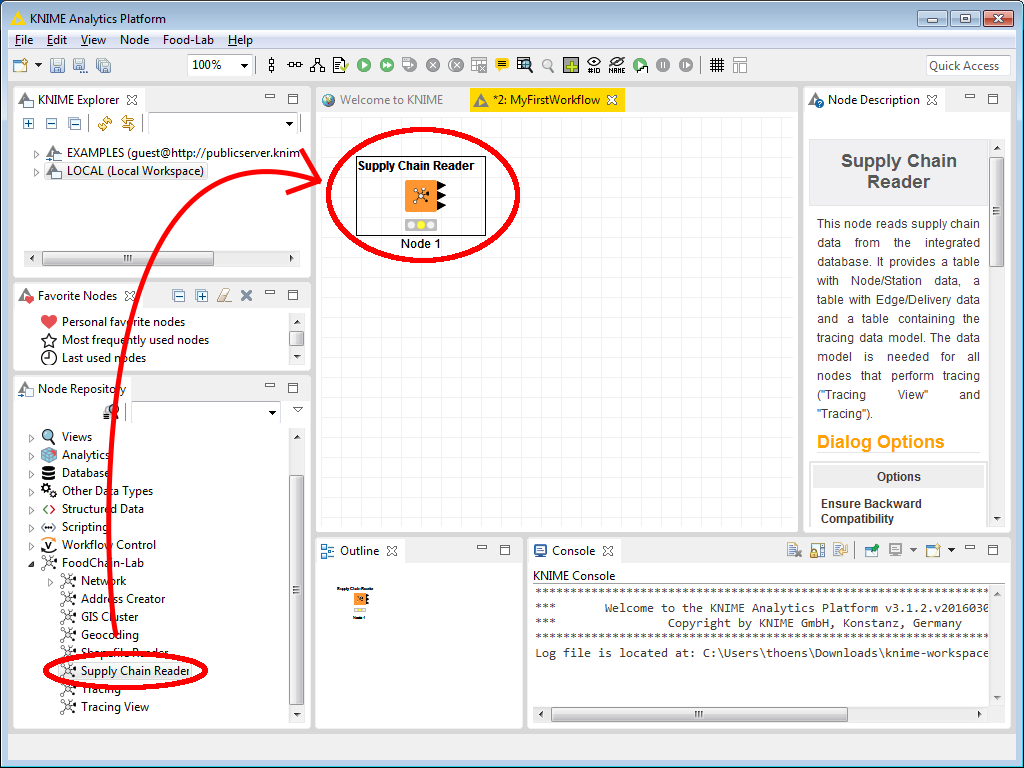
\includegraphics[height=0.6\textheight]{11.png}
	\end{center}
	\begin{itemize}
		\item Drag the \textbf{Supply Chain Reader} from the \textbf{Node Repository} to the workflow.
	\end{itemize}
\end{frame}

\subsection{12}
\begin{frame}
	\begin{center}
  		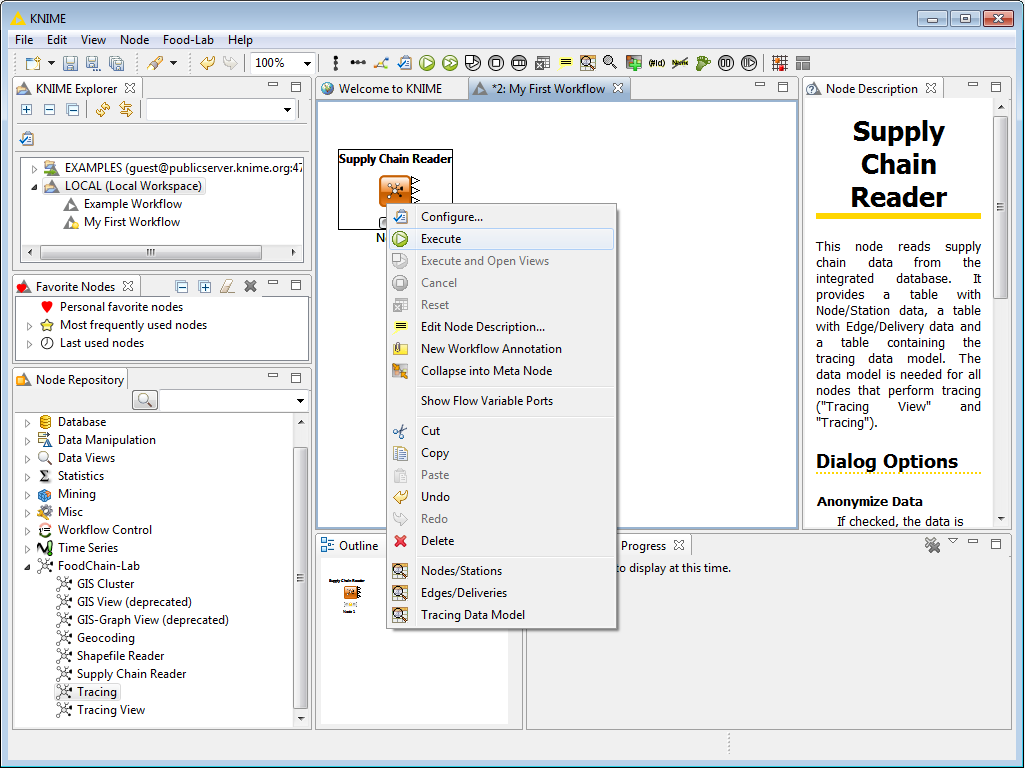
\includegraphics[height=0.6\textheight]{12.png}
	\end{center}
	\begin{itemize}
		\item We do not need to configure the \textbf{Supply Chain Reader}.
		\item Right click on it and select \textbf{Execute}.
	\end{itemize}
\end{frame}

\subsection{13}
\begin{frame}
	\begin{center}
  		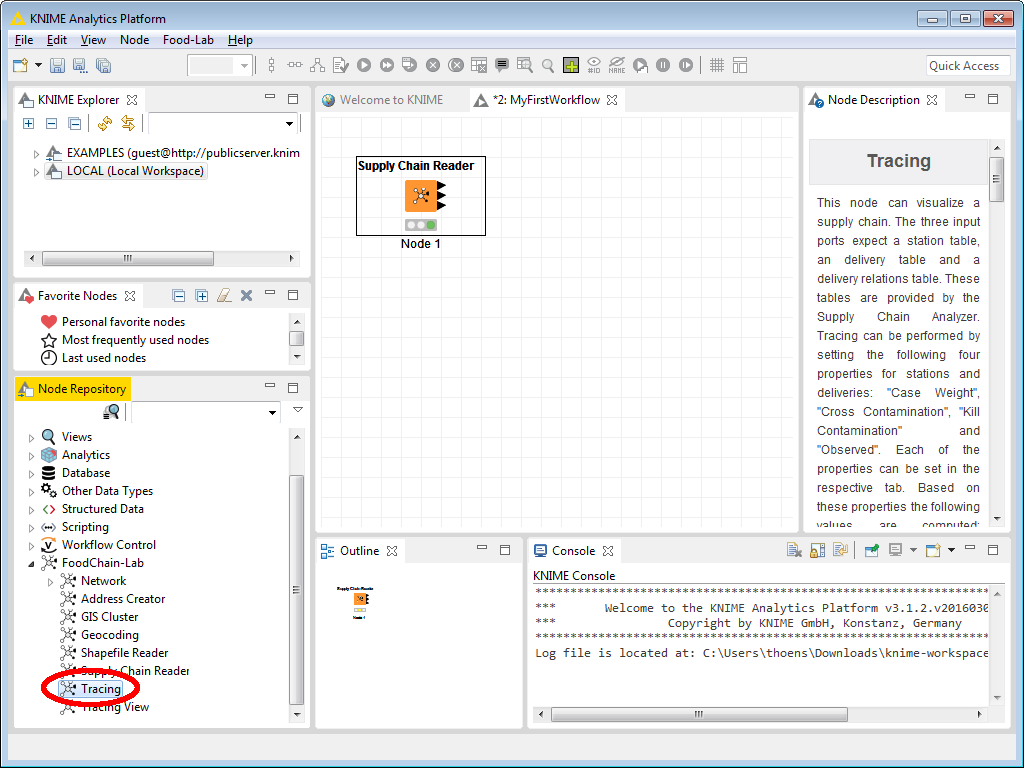
\includegraphics[height=0.6\textheight]{13.png}
	\end{center}
	\begin{itemize}
		\item The \textbf{Supply Chain Reader} has now read all data from the internal database.
		\item Select the \textbf{Supply Chain Reader} in the workflow (so that a rect is drawn around it) and double click on the \textbf{Tracing} node in the \textbf{Node Repository}.
	\end{itemize}
\end{frame}

\subsection{14}
\begin{frame}
	\begin{center}
  		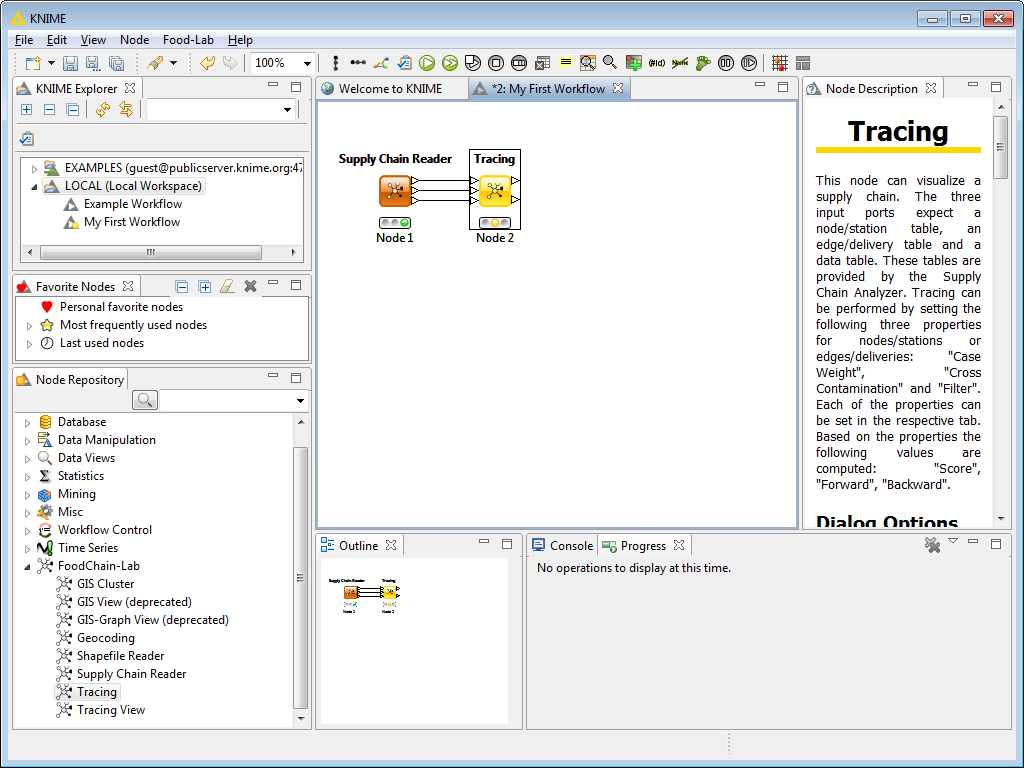
\includegraphics[height=0.6\textheight]{14.png}
	\end{center}
	\begin{itemize}
		\item The \textbf{Tracing} node should up in the workflow and its three input ports should be automatically connected to the \textbf{Supply Chain Reader}.
		\item Double click on the \textbf{Tracing} node to configure it.
	\end{itemize}
\end{frame}

\subsection{15}
\begin{frame}
	\begin{center}
  		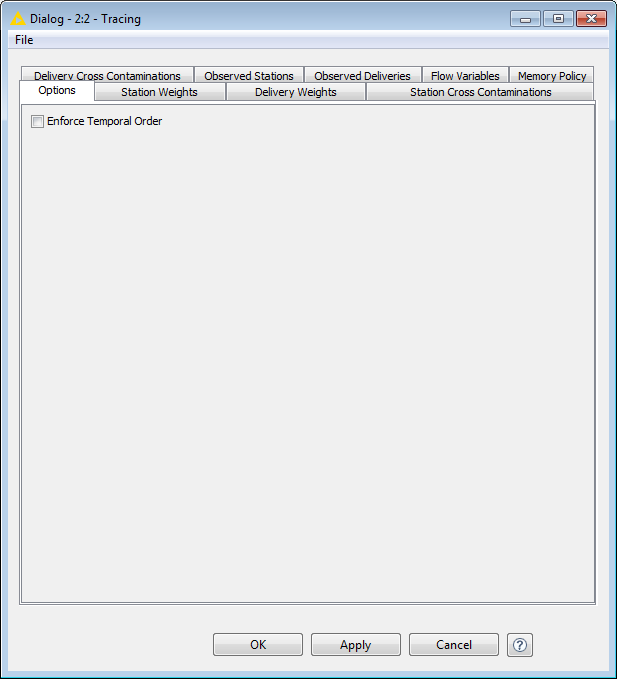
\includegraphics[height=0.6\textheight]{15.png}
	\end{center}
	\begin{itemize}
		\item You will notice several tabs for different parameters.
		\item "Weight" and "Cross Contamination" can be set for stations/deliveries. Based on these attributes a "Score" is computed for each station/delivery.
		\item Addtionally you can set "Observed" stations/deliveries.
		\item Select the \textbf{Station Weights} tab.
	\end{itemize}
\end{frame}

\subsection{16}
\begin{frame}
	\begin{center}
  		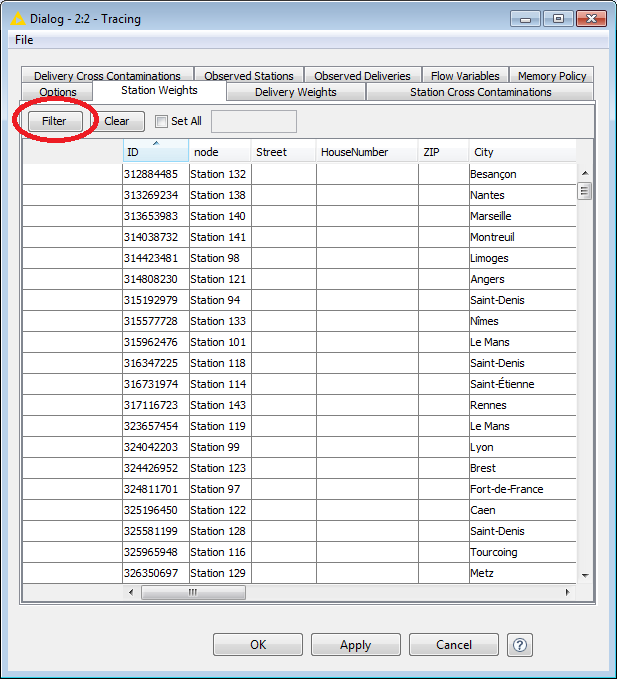
\includegraphics[height=0.6\textheight]{16.png}
	\end{center}
	\begin{itemize}
		\item A table with all available stations will pop up.
		\item The weight can be set in the left column.
		\item Since scrolling through all stations is very inefficient, we can filter out all desired stations.
		\item Click on \textbf{Filter}.
	\end{itemize}
\end{frame}

\subsection{17}
\begin{frame}
	\begin{center}
  		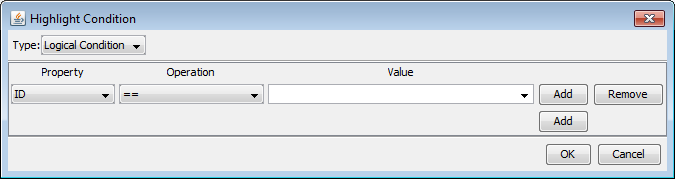
\includegraphics[width=0.9\textwidth]{17.png}
	\end{center}
	\begin{itemize}
		\item In this dialog you can specify which stations should appear in the table.
	\end{itemize}
\end{frame}

\subsection{18}
\begin{frame}
	\begin{center}
  		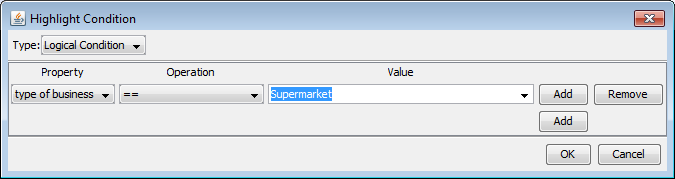
\includegraphics[width=0.9\textwidth]{18.png}
	\end{center}
	\begin{itemize}
		\item We only want to specify weights for supermarkts, since that is where contaminated products were found.
		\item Set \textbf{Property} to "type of business" and \textbf{Value} to "Supermarket".
		\item Press \textbf{OK}.
	\end{itemize}
\end{frame}

\subsection{19}
\begin{frame}
	\begin{center}
  		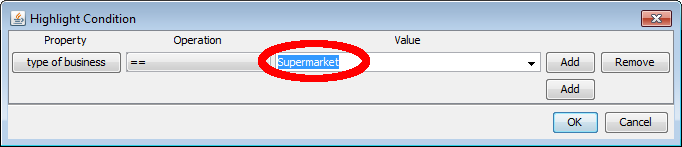
\includegraphics[height=0.6\textheight]{19.png}
	\end{center}
	\begin{itemize}
		\item Now you only see supermarkets in the dialog.
	\end{itemize}
\end{frame}

\subsection{20}
\begin{frame}
	\begin{center}
  		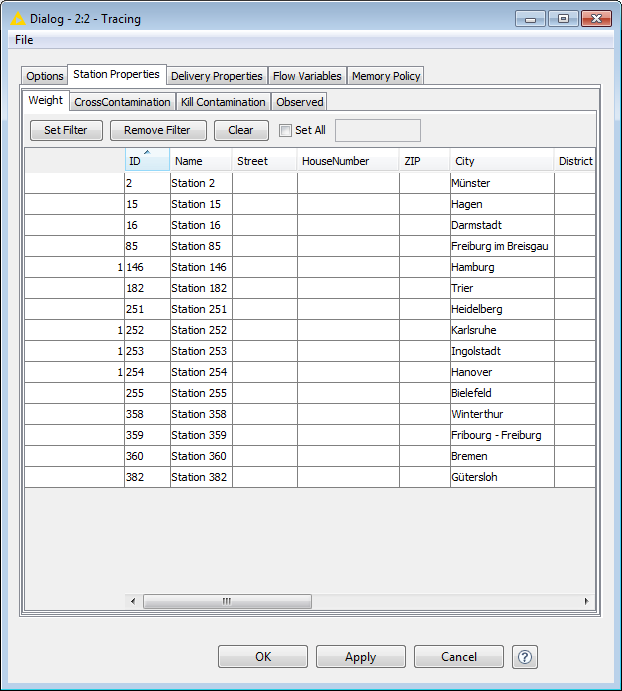
\includegraphics[height=0.6\textheight]{20.png}
	\end{center}
	\begin{itemize}
		\item Set a weight of "1" to the supermarkets in "Hamburg", "Ingolstadt" and "Münster" to indicate that contaminated products were found there.
		\item Click \textbf{OK} apply the settings and close the dialog.
	\end{itemize}
\end{frame}

\subsection{21}
\begin{frame}
	\begin{center}
  		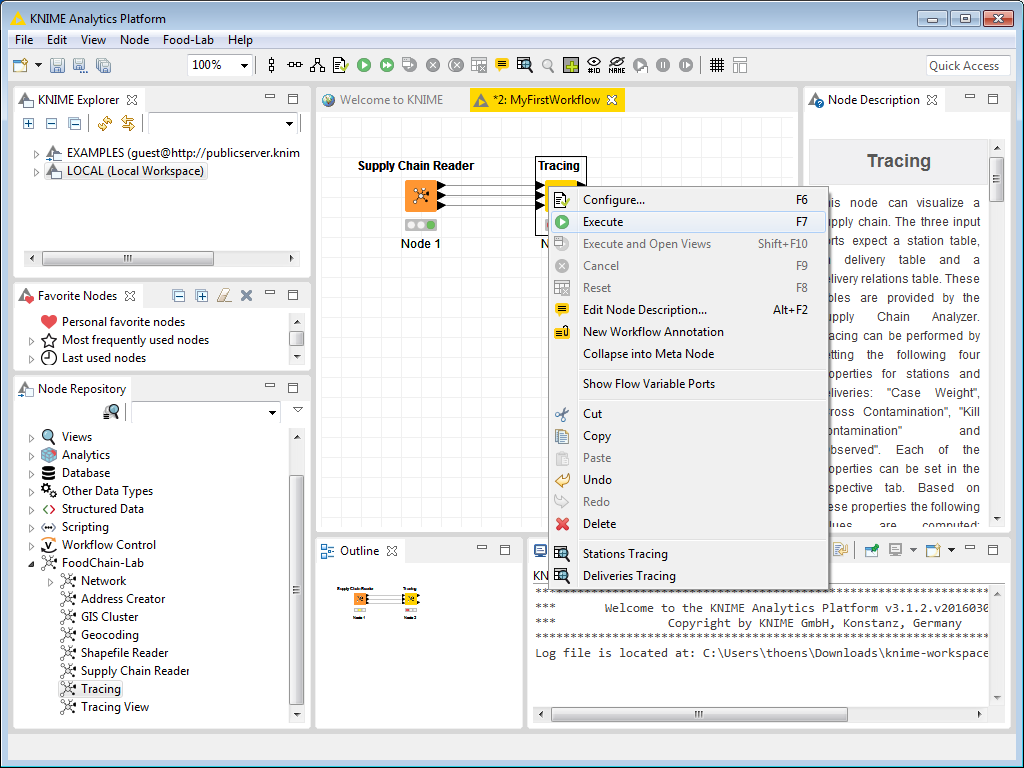
\includegraphics[height=0.6\textheight]{21.png}
	\end{center}
	\begin{itemize}
		\item Right click on the \textbf{Tracing} node and select \textbf{Execute} to execute the node.
	\end{itemize}
\end{frame}

\subsection{22}
\begin{frame}
	\begin{center}
  		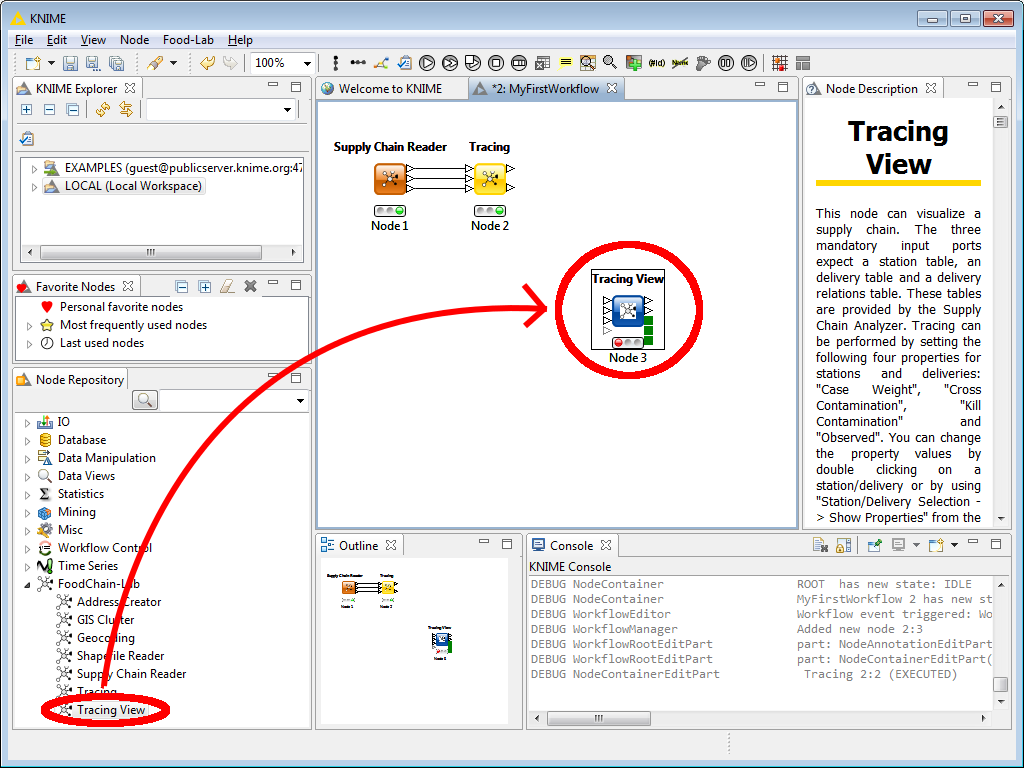
\includegraphics[height=0.6\textheight]{22.png}
	\end{center}
	\begin{itemize}
		\item Drag the \textbf{Trcing View} from the \textbf{Node Repository} to the workflow.
	\end{itemize}
\end{frame}

\subsection{23}
\begin{frame}
	\begin{center}
  		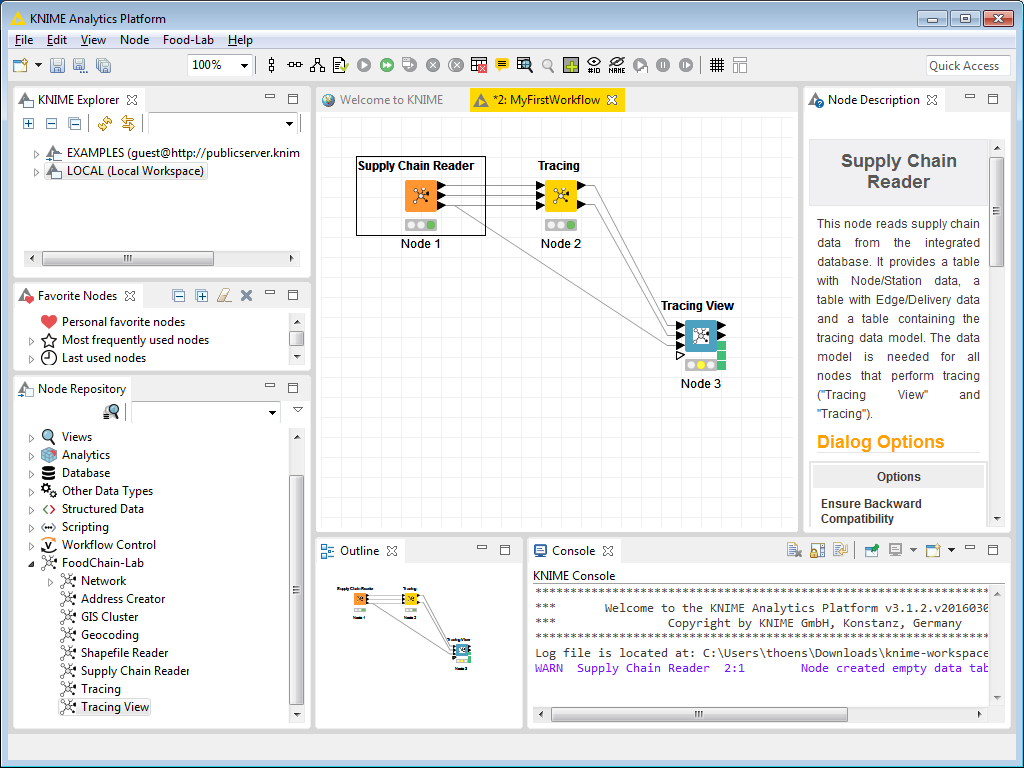
\includegraphics[height=0.6\textheight]{23.png}
	\end{center}
	\begin{itemize}
		\item Connect the output ports of the \textbf{Tracing} node to the first two input ports of the \textbf{Tracing View}.
		\item Connect the third output port of the \textbf{Supply Chain Reader} to the third input port of the \textbf{Tracing View}.
		\item Now you open the \textbf{Tracing View} and analyze the data. This will be shown in the second part of this tutorial.
	\end{itemize}
\end{frame}

\end{document}